\documentclass[USenglish,oneside,twocolumn]{article}
\usepackage{color}
\usepackage[hyphens]{url}
\usepackage{longtable}
\usepackage{graphicx}
\usepackage{enumitem}
\usepackage{pdfpages}
\usepackage{adjustbox}
\usepackage{subcaption}
%\usepackage{hyperref}

\usepackage[utf8]{inputenc}%(only for the pdftex engine)
%\RequirePackage[no-math]{fontspec}%(only for the luatex or the xetex engine)
\usepackage[big]{dgruyter_NEW}
 
\hyphenation{Isa-bela}

\DOI{foobar}

\cclogo{
\includegraphics{by-nc-nd.pdf}}

% Format a participant quotation.
\newcommand{\pquote}[2]{
\begin{quotation}
\noindent #1:~\textit{#2}
\end{quotation}
}
  
\begin{document}
  \author*[1]{Linda Lee}

  \author[2]{David Fifield}

  \author[3]{Nathan Malkin}

  \author[4]{Ganesh Iyer}

  \author[5]{Serge Egelman}
  
  \author[6]{David Wagner}

  \affil[1]{University of California, Berkeley, E-mail: \mbox{lnl@cs.berkeley.edu}}

  \affil[2]{University of California, Berkeley, E-mail: \mbox{f{}if{}ield@cs.berkeley.edu}}

  \affil[3]{University of California, Berkeley, E-mail: \mbox{nmalkin@cs.berkeley.edu}}

  \affil[4]{University of California, Berkeley, E-mail: \mbox{ganesh.v@berkeley.edu}}
  
  \affil[5]{University of California, Berkeley and International Computer Science Institute, E-mail: \mbox{egelman@cs.berkeley.edu}}
   
  \affil[6]{University of California, Berkeley, E-mail: \mbox{daw@cs.berkeley.edu}}

  \title{\huge A Usability Evaluation of Tor Launcher}

  \runningtitle{A Usability Evaluation of Tor Launcher}

  %\subtitle{...}

  \begin{abstract}
{
Although Tor has state-of-the art anti-censorship measures, users in heavily censored environments will not be able to connect to Tor if they cannot configure their connections.
We perform the first usability evaluation of Tor Launcher, the graphical user interface (GUI) that Tor Browser uses to configure connections to Tor.
Our study shows that 79\% (363 of 458) of user attempts to connect to Tor in simulated censored environments failed. We found that users were often frustrated during the process and tried options at random.
In this paper, we measure potential usability issues, discuss design constraints unique to Tor, and provide recommendations based on what we learned to help more users connect to Tor while reducing the time they take to do so. Tor Browser incorporated the changes proposed by this study.
}
\end{abstract}
  \keywords{Usable Security, User Studies, Tor, Security, Censorship, Anonymity}
%  \classification[PACS]{}
 % \communicated{...}
 % \dedication{...}

  \journalname{Proceedings on Privacy Enhancing Technologies}
\DOI{Editor to enter DOI}
  \startpage{1}
  \received{..}
  \revised{..}
  \accepted{..}

  \journalyear{2017}
  \journalvolume{2017}
  \journalissue{3}

\maketitle

\section{Introduction}
Tor~\cite{dingledine2004tor} is an anonymity network that routes Internet traffic through a series of relays 
to make it difficult to observe sources and destinations.
Tor Browser~\cite{torbrowser} is a modified Firefox browser that routes traffic through Tor, designed to minimize the configuration required before connecting.
Although Tor was originally designed for anonymity, many now use it to circumvent Internet censorship.
Because of this, many countries block Tor relays specifically to prevent their citizens from circumventing censorship~\cite{winter2012great}.

Tor Browser is bundled with a graphical configuration interface, Tor Launcher, which allows users to bypass censorship by configuring various bridges, proxies, and transport protocols prior to connecting to Tor.
Of course, these options are only effective if users understand how to use them.
To understand to what extent this is the case, we researched the effectiveness of Tor Launcher as well as how it could be improved.

Improving Tor Launcher has the obvious benefit of helping censored users connect to Tor, but this also benefits other Tor users since an increase in the overall number of users increases the anonymity set~\cite{dingledine2006anonymity}). Tor does not collect user interaction data from its real users, so we believe that usability testing research is critical to help users in heavily censored regimes and increase user adoption. In this paper, we: \\ 

\begin{itemize}
\item{Perform a qualitative and quantitative usability evaluation of Tor Launcher 5.0.3  under simulated censorship environments}
\item{Contribute design changes that improve users' likelihood of connecting to Tor and also reduce the amount of time users take to connect}
\item{Provide recommendations beyond design changes to improve Tor Launcher, such as leveraging user input (requires research) and building an automated connection scheme (requires Tor infrastructure work).}
\end{itemize} 

Specifically, we describe how the initial evaluation of the interface (Section~\ref{sec:inspection}) and our observations of participants' interactions with it (Section~\ref{sec:qualitative}).
Based on the insights from our observations, we proposed several changes to the interface (Section~\ref{sec:design}) and measured how successfully and quickly users connect to Tor before and after changes (Section~\ref{sec:quantitative}).
Finally, we provide recommendations based on what we learned (Section~\ref{sec:recommendations}), we address limitations of our evaluation (Section~\ref{sec:limitations}), and frame our study in the context of existing work (Section~\ref{sec:related}).
We hope that our usability evaluation serves as an informative case study and provides guidance on further improving Tor Launcher, as well as other privacy-enhancing technologies.


\section{Technical Background}
\label{sec:background}
This section discusses the network components involved in connecting to Tor.
An understanding of the various connection options are not required to understand our work, but we refer to these terms and methods throughout the paper.


\subsection{Proxies, Relays, Bridges, and Pluggable Transports} 

A connection to Tor involves many interacting components,
illustrated in Figure~\ref{fig:topology}.
In the presence of a local firewall and censor, it may involve a proxy and a bridge.

The word ``proxy'' has a specific meaning in the context of a Tor connection.
Generally, a proxy is any computer or service that allows users to make indirect connections to other services. In this sense, any Tor relay and the Tor circuit can also be considered a proxy. However, in this paper, the word ``proxy'' refers to a SOCKS or HTTP proxy that bypasses local firewalls.

Tor relays are the routers in the Tor network. The Tor network is a group of routers that perform onion routing, a technique for anonymous communication over a computer network.  Guard relays receive packets from the user and forward traffic to middle relays. Middle relays forward traffic from an entry relay to an exit relay. Exit relays receive traffic from a middle relay and direct the traffic to its intended destination (e.g., a website).  A user uses Tor Browser to connect to the Tor network, which connects to websites on behalf of the user. 

Bridges are unlisted alternative entry nodes used to connect to Tor when Tor relays are censored.
Bridges also receive packets from the user and forward traffic to middle relays, but may also run a pluggable transport (referred to as ``transport'' for shorthand). Pluggable transports specify alternative protocols by which Tor Browser may connect to the Tor network, thereby disguising Tor traffic to make it harder to detect and block bridges.
When a bridge is used, it takes the place of the guard relay.
For convenience, bridges are grouped in the interface by which transport they run.

Tor Launcher is the graphical user interface for configuring
an optional proxy, bridge, and transport
prior to initiating a connection to the Tor network.
Figure~\ref{fig:old-interface} shows the various screens
of Tor Launcher at the time we began our research.

Most bridges can be blocked by blocking their static IP addresses. These include bridges that run the \texttt{fte} and \texttt{fte-ipv6}~\cite{fte} pluggable transports, which disguise the Tor protocol as another protocol (such as HTTP); these also include the \texttt{obfs3}~\cite{obfs3}, \texttt{obfs4}~\cite{obfs4}, and \texttt{scramblesuit}~\cite{scramblesuit} transports, which encrypt or alter the Tor protocol to appear as random noise.

Other bridges are less susceptible to blocking because of how they work. Bridges that run the \texttt{flashproxy}~\cite{flashproxy} and \texttt{meek}~\cite{fifield2015blocking} transports route traffic through third party web browsers and content delivery networks. The bridges and transports that are accessible in each country vary. Figure~\ref{fig:old-bridge-combobox} shows the bridge and transport options at the time of our study.

\begin{figure}
\centering

\includegraphics{topology.pdf}
\caption{
The chain of components involved in connecting to a website over Tor.
Most users do not need a proxy;
only users who face a censor need a bridge.
In the diagram, ``Tor'' represents a circuit of hops through the Tor network.
We have shown the bridge as a separate component
because of the special role it plays.
When a bridge is used, it becomes the first Tor relay.
}
\label{fig:topology}
\end{figure}

\subsection{Connecting to Tor} 
It is important to note that there are many valid configuration settings that can be used to connect to the Tor network. A user may or may not need a proxy and/or a bridge.
A user who does not need a bridge or proxy can still connect with a bridge, proxy, or both, provided that these are configured correctly (though adding unnecessary network hops or obfuscation protocols may slow the connection down).

Users can configure a bridge by choosing a transport, which selects the group of bridges that use that transport.
For instance, a user choosing the \texttt{obfs3} option in Figure~\ref{fig:old-bridge-combobox} will be assigned one of these bridges as their guard relay.
If these built-in options do not work, users can obtain bridge configurations through out-of-band channels~\cite{bridgedb}.
Configuring a proxy requires entering in the proxy protocol, IP address, port, and additional optional fields (Figure~\ref{fig:old-proxy}).
The user must obtain this information themselves.

\begin{figure*}
\centering
\begin{subfigure}[b]{0.30\textwidth}
	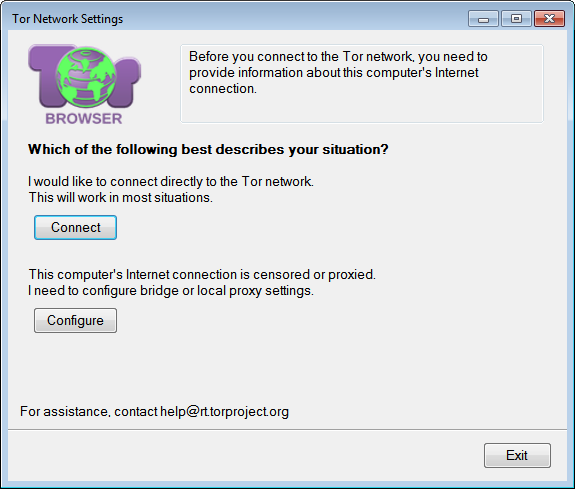
\includegraphics[width=\textwidth]{screenshots/OLD-first.png}
	\centering\captionsetup{width=1.5\linewidth}%
	\caption{The first screen (F). ``Connect'' starts a connection. ``Configure'' leads to the first bridge screen (Figure~\ref{fig:old-bridge}). }
	\label{fig:old-first}
\end{subfigure}
~~~~~~~~~~~~~~~~~~~~~~~~~
\begin{subfigure}[b]{0.30\textwidth}
	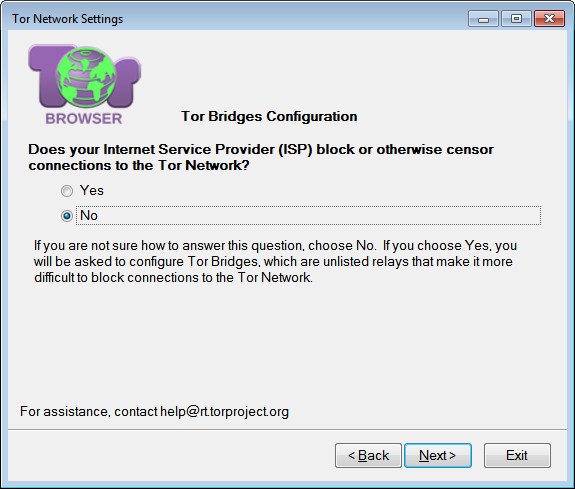
\includegraphics[width=\textwidth]{screenshots/OLD-bridges.png}
	\centering\captionsetup{width=1.5\linewidth}%
	\caption{The first bridge screen (B1). ``Yes'' leads to a bridge configuration screen (Figure~\ref{fig:old-bridge-settings}) and ``no'' skips to P1.}
	\label{fig:old-bridge}
\end{subfigure}
~~~~~~~~~~
\begin{subfigure}[b]{0.30\textwidth}
	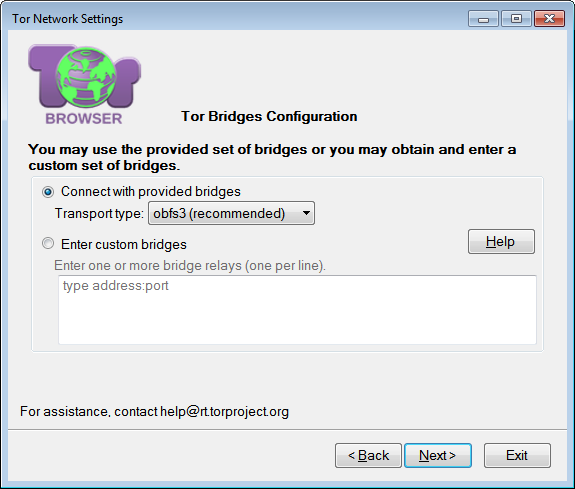
\includegraphics[width=\textwidth]{screenshots/OLD-bridgeSettings.png}
	\centering\captionsetup{width=1.5\linewidth}%
	\caption{The second bridge screen (B2). Users select a bridge here. ``Help'' directs to bridge help screen (Figure~\ref{fig:old-bridge-help}). }
	\label{fig:old-bridge-settings}
\end{subfigure}
~~~~~~~~~~~~~~~~~~~~~~~~~
\begin{subfigure}[b]{0.30\textwidth}
	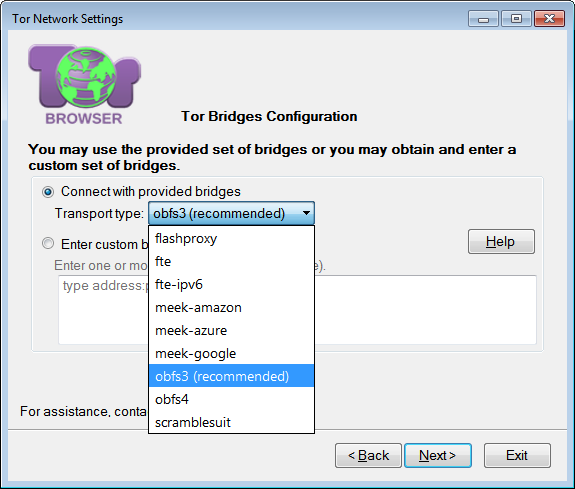
\includegraphics[width=\textwidth]{screenshots/OLD-bridgeSettings-combobox.png}
	\centering\captionsetup{width=1.5\linewidth}%
	\caption{Some hardcoded bridges are listed alphabetically by their transport. The recommended one is obfs3.}
	\label{fig:old-bridge-combobox}
\end{subfigure}
~~~~~~~~~~
\begin{subfigure}[b]{0.30\textwidth}
	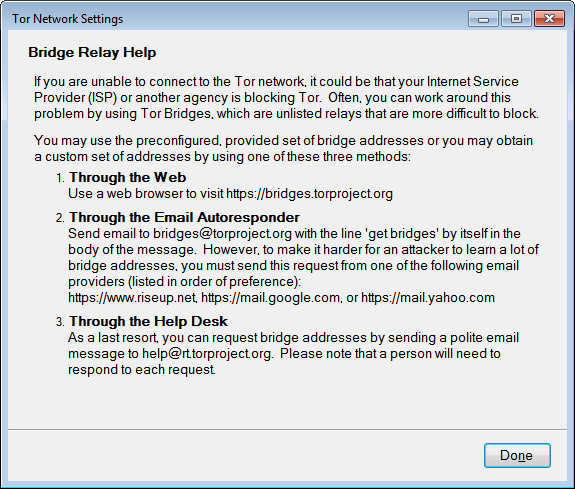
\includegraphics[width=\textwidth]{screenshots/OLD-bridgeHelp.png}
	\centering\captionsetup{width=1.5\linewidth}%
	\caption{The bridge help screen (BH) talks about getting a custom bridge. ``Done'' leads back to the previous screen.}
	\label{fig:old-bridge-help}
\end{subfigure}
~~~~~~~~~~~~~~~~~~~~~~~~~
\begin{subfigure}[b]{0.30\textwidth}
	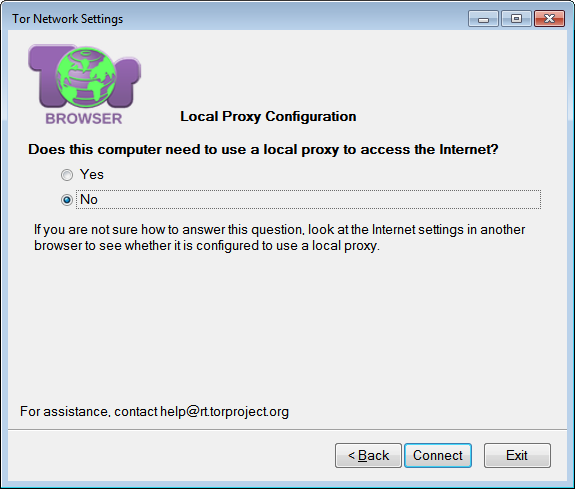
\includegraphics[width=\textwidth]{screenshots/OLD-proxy.png}
	\centering\captionsetup{width=1.5\linewidth}%
	\caption{The proxy question screen (P1). ``Yes'' goes to the proxy settings screen (Figure~\ref{fig:old-proxy-yes}). and ``no'' starts a connection.}
	\label{fig:old-proxy}
\end{subfigure}
~~~~~~~~~~
\begin{subfigure}[b]{0.30\textwidth}
	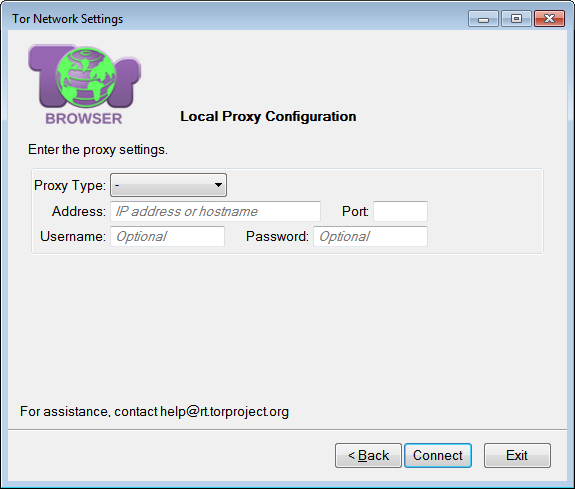
\includegraphics[width=\textwidth]{screenshots/OLD-proxyYES.png}
	\centering\captionsetup{width=1.5\linewidth}%
	\caption{The proxy settings screen (P2). ``Connect'' starts a connection to Tor with the interface settings.}
	\label{fig:old-proxy-yes}
\end{subfigure}
~~~~~~~~~~~~~~~~~~~~~~~~~
\begin{subfigure}[b]{0.30\textwidth}
	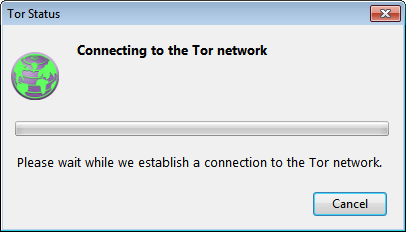
\includegraphics[width=\textwidth]{screenshots/OLD-progress.png}
	\centering\captionsetup{width=1.5\linewidth}%
	\caption{The progress bar (Pr). The bar fills up as log messages update the connection status. }
	\label{fig:old-progress}
\end{subfigure}
\caption{
The Tor Browser 5.0.3 Tor Launcher GUI. Screens are in the order that they appear. 
}
\label{fig:old-interface}
\end{figure*} 

\section{Methodology} 
This section discusses our usability testing process, including the simulated censorship environments we used to require users to configure different network components to connect to Tor and the evaluation metrics  we collected.

\subsection{Testing Pipeline} 
We began by performing a cognitive walkthrough~\cite{wharton1994cognitive,cognitive-walkthrough} to inspect the interface to anticipate potential problems and formally assess its pros and cons.
A cognitive walkthrough is a formal method of inspection performed by researchers without any user involvement.
We then conducted qualitative and quantitative usability tests.
We believe both methods were necessary for a complete usability evaluation.
Qualitative testing illuminates {\it why or how} the software is or is not usable, while quantitative testing measures {\it to what extent}.
We used our observations from the qualitative study to design interface changes that would address common issues that participants encountered.
We used our quantitative testing setup to measure the usability of our proposed changes, as compared to the original interface.

We performed our qualitative experiments one participant at a time, so that we could observe their behaviors in real time and interview them about their experience after user.
We recruited five participants per experimental condition to gather qualitative data; this is considered the optimal number of measurements to maximize the cost-benefit ratio~\cite{howmanyusers}.
We performed our quantitative experiments at a behavioral laboratory many participants at a time, using instrumentation to capture evaluation metrics.
We recruited twenty users per experimental condition to gather quantitative data; this is considered to be the minimum for yielding statistically significant measurements~\cite{howmanyusers}.

\subsection{Experimental Setup}
\label{sec:environments}
We chose to simulate environments for the stability and reproducibility of the experiment, as real censored networks are volatile and complex. Re-routing participant traffic through other countries' networks also may introduce unforeseen risks to the participants out of our control and performing hundreds of connections in short intervals during experiments may draw unnecessary attention to Tor use in that country. The three environments are described in Table~\ref{tab:environments}.

\begin{table}[t]
\centering
\begin{tabular}{r c c c}
& E1 & E2 & E3 \\
% \noalign{\hrule}
websites blocked & X & X & X \\
public relays blocked & & X & X \\
default bridges blocked & & & X \\
\end{tabular}
\caption{
Summary of our simulated censorship environments.
E1 only requires users to connect directly;
E2 requires users to connect with a built-in bridge;
and E3 requires users to connect with a specific type of built-in bridge
or a custom bridge.
E2's blocking is a superset of E1's;
similarly, E3's is a superset of E2's.
}
\label{tab:environments}
\end{table}

The simulated environments are not intended to imitate any particular country's network---though they do use the same techniques that are currently used by various censorship regimes. Rather, we designed simulated environments to have different requirements to connect to Tor. We believe this to be sufficient for the purpose of testing the configuration interface, since this requires the user to take the different interface paths we wanted to test (and matches the actions real users would need to take to circumvent various types of censorship).

In the first environment, E1, particular websites were blocked, which meant that they could be accessed using a default Tor configuration (i.e., bridges or proxies were not needed). In the second environment, E2, we additionally blocked the IP addresses of public Tor relays, which meant that Tor could still be accessed by enabling any of the included bridges. Finally, the third environment, E3, additionally blocked several of the included bridges, which required experimenting with several different bridges---beyond the recommended option---in order to successfully connect.

The simulated environments are not intended to imitate any particular country's network---though they do use the same techniques that are currently used by various censorship regimes. Rather, we designed simulated environments to have different requirements to connect to Tor. We believe this to be sufficient for the purpose of testing the configuration interface, since this requires the user to take the different interface paths we wanted to test (and matches the actions real users would need to take to circumvent various types of censorship).

We used Tor Browser~5.0.3, the most recent stable release at the time~\cite{torbrowser-503}.
There were new releases during the experiments, but we used the same version throughout to not introduce confounding factors. We conducted our experiments on Windows machines. To create the environments, we used Windows Firewall rules to block the IP addresses of public Tor relays and default bridges, and the Windows hosts file to block websites by mapping domain names to localhost. 

\subsection{Evaluation Metrics}
\label{sec:eval}
We use the following three industry-standard~\cite{albert2013measuring} usability metrics to quantify how easily users completed their task and if they were productive with their time: \\

\begin{itemize}
\item {\bfseries Completion rate:}  the percentage of users that want to connect to Tor and successfully do so. The higher the completion rate, the better. The ideal case would be that everyone is able to connect to Tor if they want to. Even if users do not successfully connect to Tor at first but eventually do so during the experiment, they are considered to have successfully connected to Tor for this metric.
\item {\bfseries Connection time:} the amount of time users take to connect to Tor. The less time it takes for users to connect, the better. The ideal case would be that the connection time is very close to the time it takes for the application to communicate with the servers and establish a circuit of relays for the connection, which can take up to several minutes. Connection time includes this bootstrapping time and any additional time that people spend in the interface.
\item {\bfseries Configuration time:} the amount of time users spend in the interface. The less time it takes for users to configure their preferences, the better. Configuration time is included in connection time, so it will always be less than connection time. We defined configuration time as any time spent on the bridge and proxy screens, since users were most likely configuring bridges and proxies. We excluded any time spent on the progress screen, because users were most likely waiting for connections to establish or timeout and not necessarily interacting with the interface. This should be as short as possible.
\end{itemize}

Completion rate is the most important usability metric, measuring if users can accomplish the task. We defined success as a binary metric that is true if a user connected to Tor and false if a user did not.
Task time is a supplemental usability metric that measures user productivity during the task. We use both connection and configuration time to quantify productivity since the bootstrapping time, and hence, time spent waiting for the connection to succeed or fail, can dominate the measurement.


\section{Cognitive Walkthrough}
\label{sec:inspection}
We inspected the interface to anticipate potential problems before testing it on study participants.

\subsection{Procedure} 
Two researchers performed the cognitive walkthrough~\cite{cognitive-walkthrough} on the Tor Browser 5.0.3 Tor Launcher GUI, which was the most recent version deployed at the time (Figure~\ref{fig:old-interface}). We first examined each screen in the interface for tasks required, inputs taken, and consequences of possible actions. This was done to map all potential paths through the interface (Figure~\ref{fig:digraph}). We then stepped through each user path, systematically tried all possible actions, and recorded our observations. 

\subsection{Observations}
We noticed that the interface leaves a lot of freedom for error while not giving good instructions on how to recover from errors: \\

\begin{itemize}
\item {\bfseries Technical terms:} The interface uses technical and Tor-specific terms that are likely unfamiliar to an average user (e.g., ``Tor network,'' ``local proxy,'' ``bridges,'' and ``transports''). 
\item {\bfseries Too many choices:}  Users who do not need a bridge or proxy are able to configure them.
There are nine choices for bridges and more options to input a custom bridge.
Almost any HTTP or SOCKS proxy can be used as the proxy.
Custom bridge lines require the bridge information in a specific syntax, but this syntax is not specified in the interface.
Proxy fields also do not provide syntactic guidelines.
The full list of possible errors we identified can be found in Appendix~\ref{states}.
\item {\bfseries Poor feedback:} Even if there was a syntactic error in the bridge or proxy fields, the user is not notified until after a connection is attempted and fails. If a censored bridge was chosen, the connection timeout takes several minutes. Error messages were often technical and did not give suggestions for next steps.
\end{itemize}

These are some of the factors that we believed contribute to users struggling with the interface and therefore may prevent them from connecting to Tor quickly.


\begin{figure*}
\centering
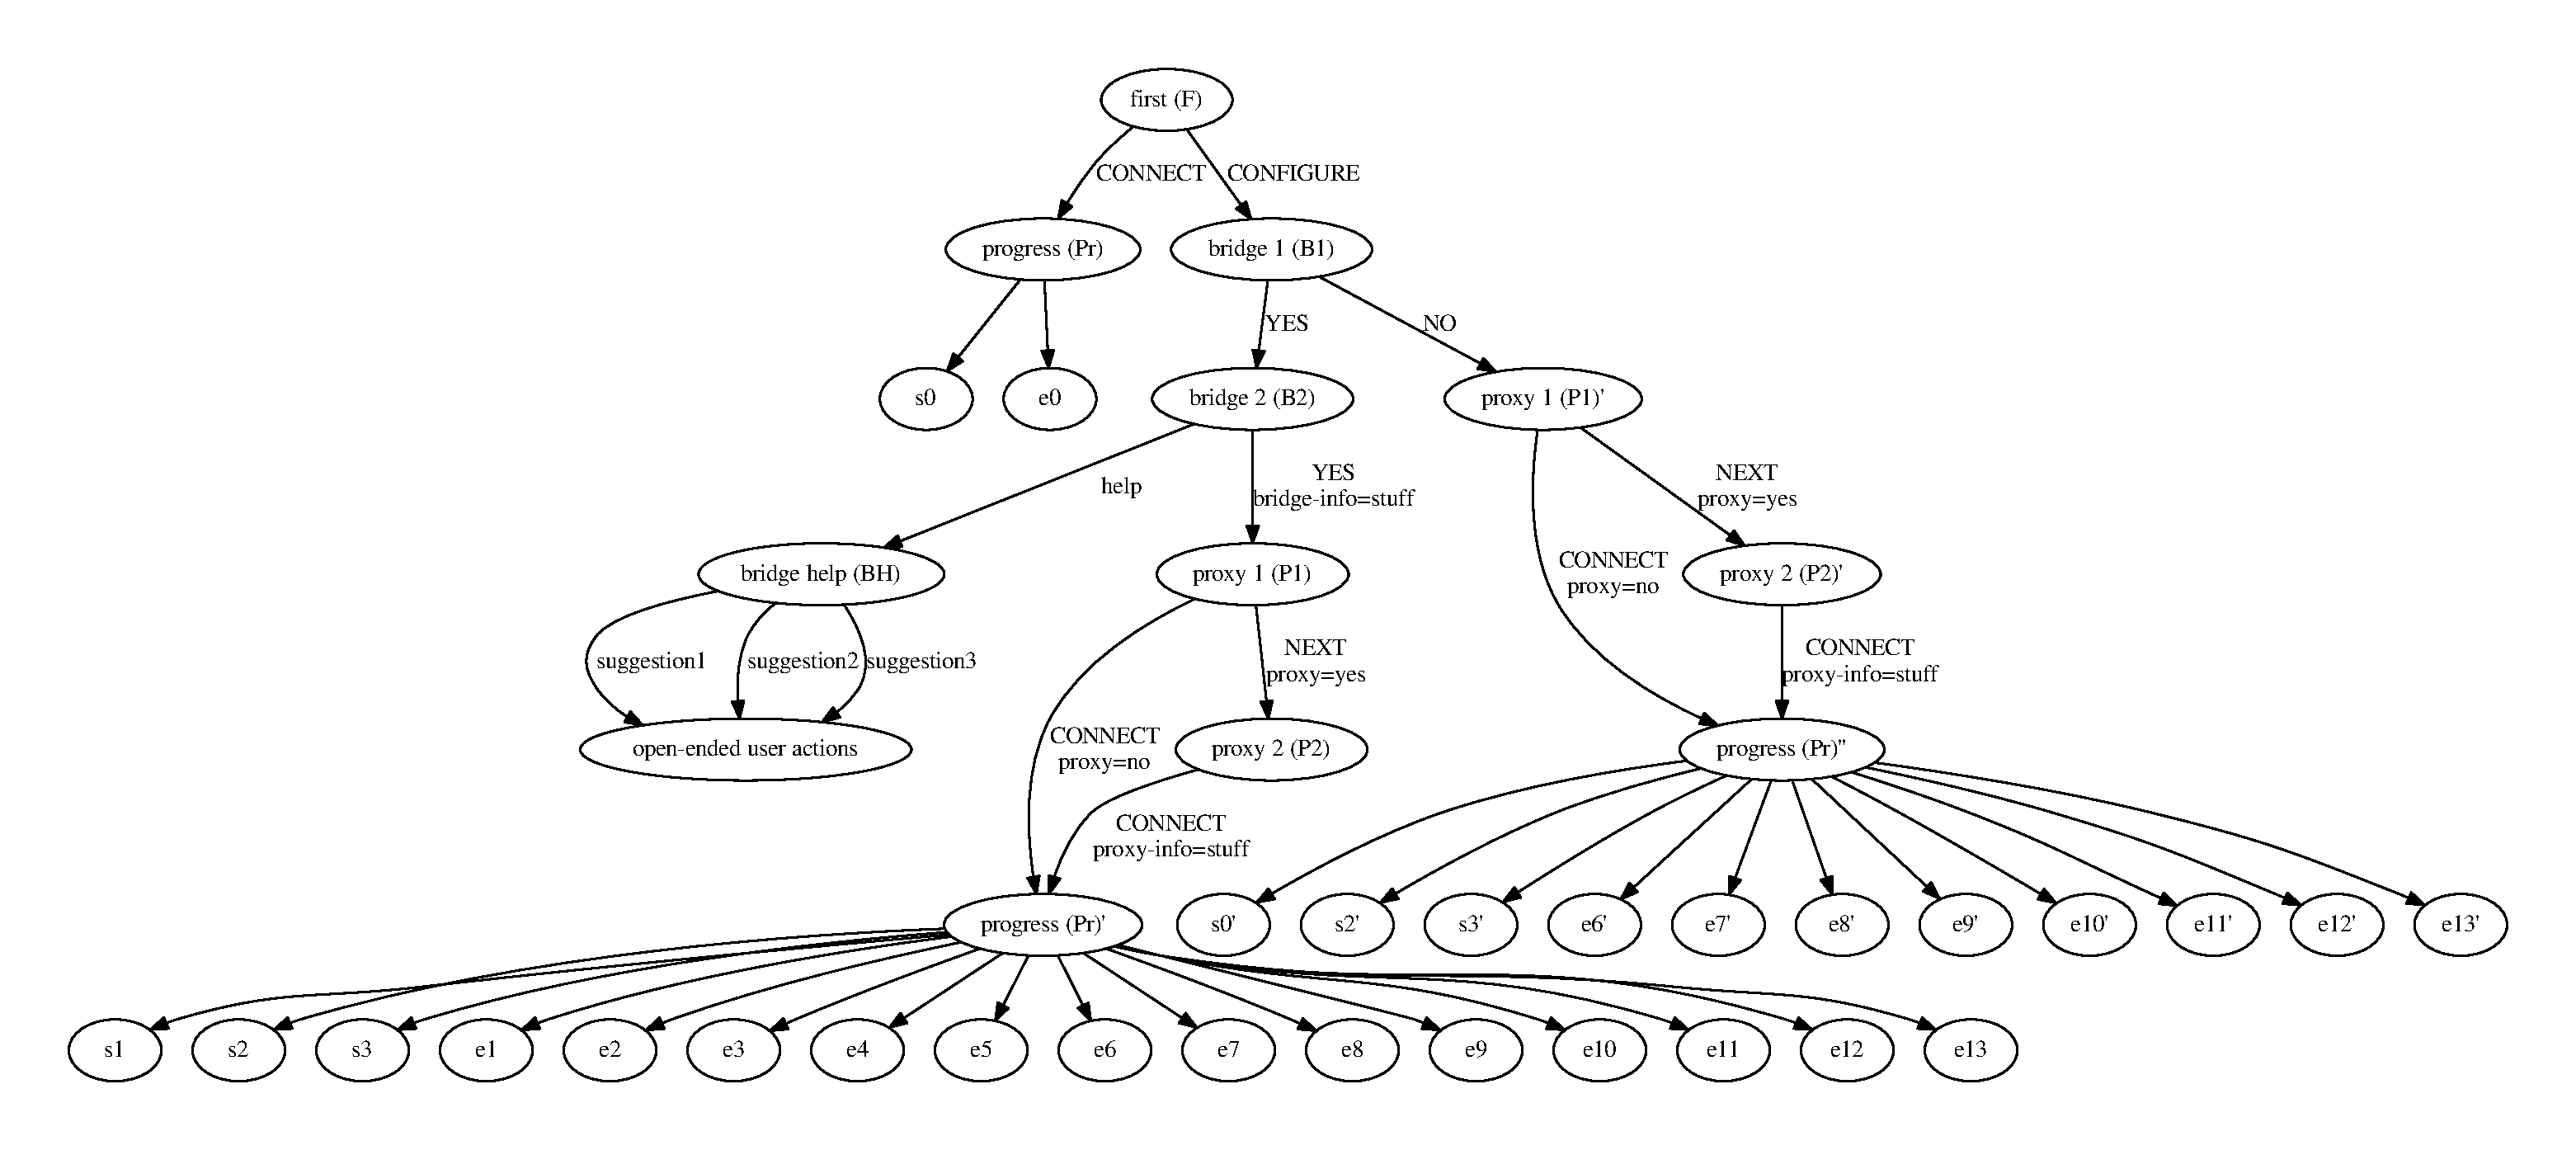
\includegraphics[width=\textwidth]{torconfig.pdf}
\caption{
A digraph illustrating the potential user paths through the interface. Non-leaf nodes are screens in the user interface (start, bridge 1, bridge 2, proxy 1, proxy 2, and progress). Leaf nodes are various end states (quit, success, or error). Transitions between these nodes denote user actions. 
}
\label{fig:digraph}
\end{figure*} 

\section{Qualitative Testing}
\label{sec:qualitative}
We performed our qualitative experiments one participant at a time, so that we could observe their behaviors in real time identify stumbling points in the interface.
At the completion of the task, we interviewed our participants to gather explanatory data and their opinions.

\subsection{Recruitment}
We recruited people from Craigslist using an ad (Appendix~\ref{qualitative-recruitment}) and prescreening survey (Appendix~\ref{qualitative-prescreening}). We pre-screened~\cite{screening} so that we could have a diversity of gender, age, and familiarity with Tor in a small participant pool. Of our 16 recruited participants, 50\% identified as male and 50\% identified as female. Ages ranged from 20 to~62 years ($\mu = 30.5$, $\sigma = 13.5$). Our age statistics omit one participant who declined to disclose their age. All of our participants had at least some college education. Twelve were new users and four had previously used Tor Browser in some capacity.  

% gender: Male: 8/Female: 8
% education: At least some college 16
% ages: 22, 23, 34, 52, 25, 22, 29, 21, 25, didn't answer, 20, 20, 26, 24, 62, 52


As we performed the experiments, we distributed participants evenly across experimental conditions:  5~in E1, 5~in E2, and 6~in E3. We ensured that each condition had new and previous Tor Browser users, and tried for variation in gender and age.

\subsection{Procedure} 
We ran the experiments in a small room with a desk and chair, where a monitor, keyboard, and a Windows computer were set up. On a clean computer, we installed Tor Browser 5.0.3 for testing, Chrome, Firefox, and Internet Explorer as browser options, and VLC media player~\cite{vlc} to record the screen during the experiment. We ran a script that set up one of the three simulated environments (E1, E2, or E3) and started recording the computer screen before each participant.

We get informed consent by talking about the study, task, and risks (Appendix~\ref{qualitative-script}). Then the participant visited sample websites in a non-Tor browser to illustrate that some sites were blocked and instruct them to use Tor to circumvent censorship. Their task was to complete a worksheet (Appendix~\ref{participant-worksheet}) that required visiting a censored website (Wikipedia) and an uncensored website (CNN). We chose Wikipedia and CNN because their likely familiarity~\cite{alexa}. After giving the instructions, the researchers left the room to minimize interactions and watched a live feed of the participant's screen.

After 45 minutes (or when participants finished the worksheet), we interviewed the participant about their experience. We asked general questions (Appendix~\ref{interview-questions}) and participant-specific questions to verify any observations (e.g., ``the participant was selecting bridges at random''). After the interview, we allowed the participant to ask any questions about the experiment, then gave them~\$30 for their time. 

\subsection{Results} 

Here we report about the main reasons why participants struggled to use Tor launcher, summarizing general behavioral trends and attitudes. 

\subsection{Pain Points in Tor Launcher} 
\label{sec:pain-points}
Participants spent a lot of time going back and forth on screens, looking for proxy information, and waiting for the connection to work or time out. We believe that the reasons for these behaviors were:\\

\begin{itemize}
\item {\bfseries Unfamiliar concepts:} Participants found technical terms (i.e. relay, bridge, proxy, censor, ISP) confusing, and were often unable to answer the questions that were designed to guide them (Figures~\ref{fig:old-bridge} and~\ref{fig:old-proxy}).
\end{itemize} 

%P11 in the repo, P9 in the paper
\pquote{P9}{``You can only answer this question correctly if you know what a local proxy is.
Otherwise you have no chance...''}

%P13 in the repo, P7 in the paper 
\pquote{P7}{``[I] was just fiddling, to be honest with you... it was kind of confusing.''}

\begin{itemize}
\item {\bfseries Missing information:} They did not know how to choose a bridge by transport or which bridges worked in their environment (Figures~\ref{fig:old-bridge-combobox}).
\end{itemize} 

%P8 in the repo, P10 in the paper
\pquote{P10}{``I have no clue what's the difference between flashproxy, fte, etc. And why do I need a custom bridge if there are options built in?''}

\begin{itemize}
\item {\bfseries Bad recovery:} Participants had to wait a couple minutes to know if their connection failed, and also were quite upset that they had to wait that long to find out that their connection failed.
\end{itemize} 

%P16 in the repo, P13 in the paper
\pquote{P13}{``Put in a 30 second timeout! I don't know, maybe it takes longer than that...''}

%P1 in the repo, P15 in the paper
\pquote{P15}{``there doesn't seem to be any timeout on any of this stuff. Am I waiting long enough? Should I wait 5 minutes?''}

These were our general observations. Participants who could connect directly (E1) or use the recommended bridge had an easy time connecting (E2), but the participants who could not use many of the hardcoded bridges (E3) did not know what to do. For a summary of how each participant connected to Tor and what behavioral trends dominated in each environment, see Appendix~\ref{summary}. 

\section{Interface Redesign}
\label{sec:design} 
We redesigned the interface according to usability best practices while addressing the pain points found in our qualitative usability study. We drafted a list of design considerations, prioritized the pain points to address, and iteratively made changes to the interface to get to our final design (Figure~\ref{fig:new-interface}).

\begin{figure*}
\centering
\begin{subfigure}[b]{0.30\textwidth}
	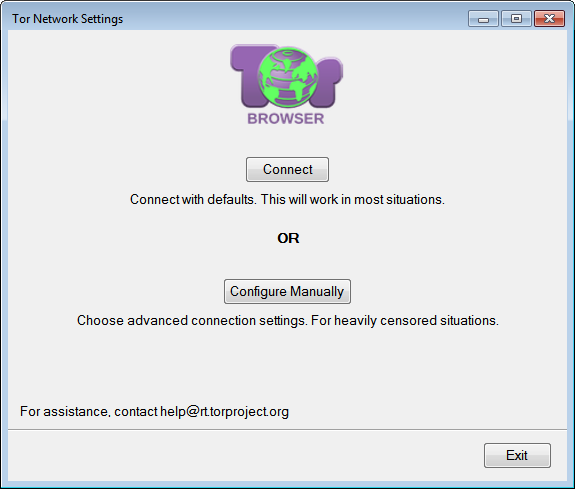
\includegraphics[width=\textwidth]{screenshots/NEW-first.png}
	\centering\captionsetup{width=1.5\linewidth}%
	\caption{The first screen (F) with reduced, alternative text. We said configuration was required for heavy censorship.}
	\label{fig:new-first}
\end{subfigure}
~~~~~~~~~~~~~~~~~~~~~~~~~
\begin{subfigure}[b]{0.30\textwidth}
	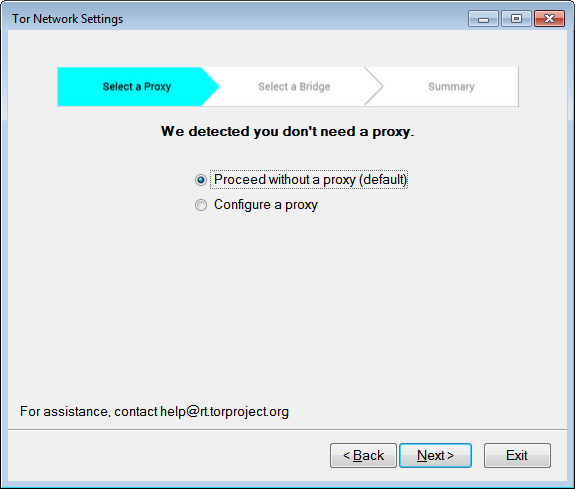
\includegraphics[width=\textwidth]{screenshots/NEW-proxyYES.png}
	\centering\captionsetup{width=1.5\linewidth}%
	\caption{The proxy screen (P). The interface locally detects a proxy and automatically populates the fields as necessary.}
	\label{fig:new-proxy}
\end{subfigure}
~~~~~~~~~~
\begin{subfigure}[b]{0.30\textwidth}
	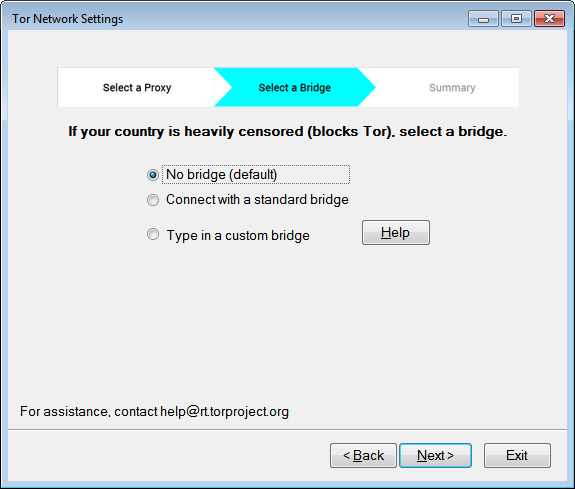
\includegraphics[width=\textwidth]{screenshots/NEW-bridgeSettings.png}
	\centering\captionsetup{width=1.5\linewidth}%
	\caption{The bridge screen (B). We give users the options to connect with or without a bridge all on one screen, and eliminated the bridge question screen.}
	\label{fig:new-nobridge}
\end{subfigure}
~~~~~~~~~~~~~~~~~~~~~~~~~
\begin{subfigure}[b]{0.30\textwidth}
	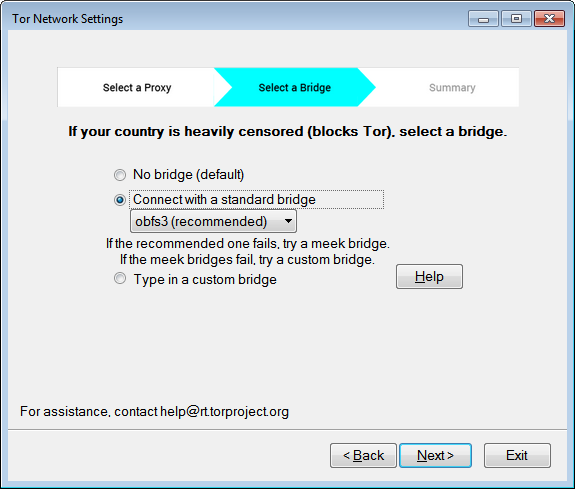
\includegraphics[width=\textwidth]{screenshots/NEW-bridgeSettings-default.png}
	\centering\captionsetup{width=1.5\linewidth}%
	\caption{The bridge menu and additional advice shows up when the corresponding option is chosen. The custom bridge input fields are hidden until the custom option is chosen.}
	\label{fig:new-bridge}
\end{subfigure}
~~~~~~~~~~
\begin{subfigure}[b]{0.30\textwidth}
	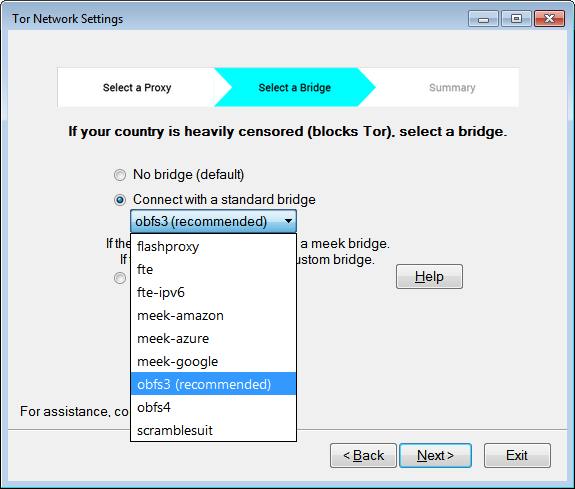
\includegraphics[width=\textwidth]{screenshots/NEW-bridgeSettings-combobox.png}
	\centering\captionsetup{width=1.5\linewidth}%
	\caption{This dropdown menu remains the same (see Figure~\ref{fig:old-bridge-combobox}).}
	\label{fig:new-bridge-combobox}
\end{subfigure}
~~~~~~~~~~~~~~~~~~~~~~~~~
\begin{subfigure}[b]{0.30\textwidth}
	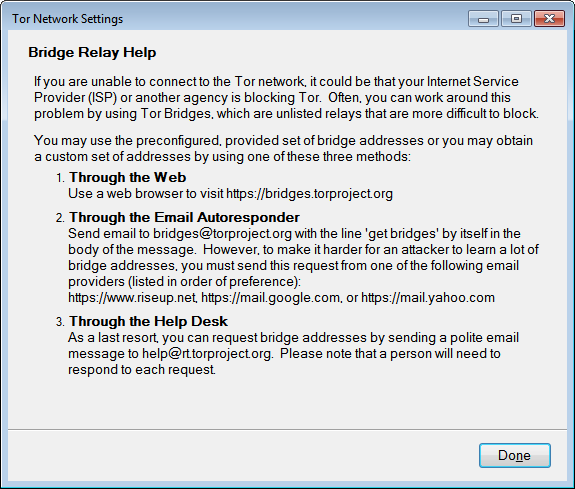
\includegraphics[width=\textwidth]{screenshots/NEW-bridgeHelp.png}
	\centering\captionsetup{width=1.5\linewidth}%
	\caption{The bridge help screen (BH) remains the same as well.}
	\label{fig:new-bridge-help}
\end{subfigure}
~~~~~~~~~~
\begin{subfigure}[b]{0.30\textwidth}
	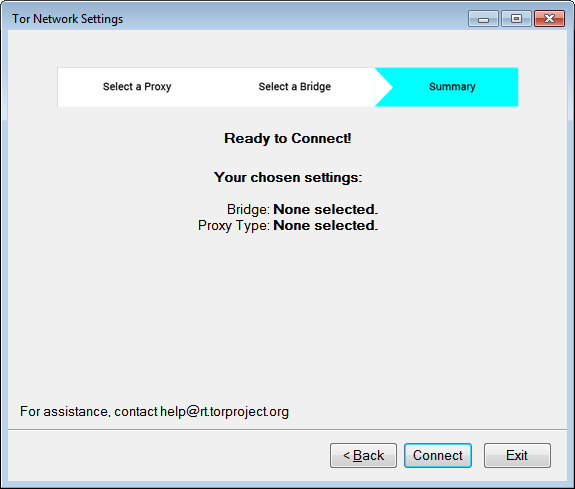
\includegraphics[width=\textwidth]{screenshots/NEW-summary.png}
	\centering\captionsetup{width=1.5\linewidth}%
	\caption{The summary screen (S) summarizes the configuration. This example configuration is connecting directly to Tor.}
	\label{fig:new-summary}
\end{subfigure}
~~~~~~~~~~~~~~~~~~~~~~~~~
\begin{subfigure}[b]{0.30\textwidth}
	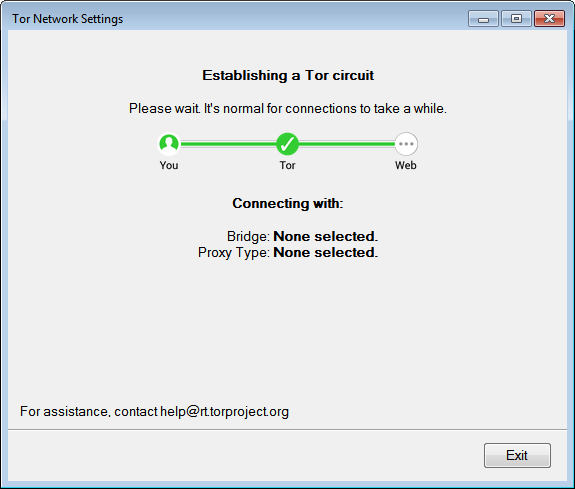
\includegraphics[width=\textwidth]{screenshots/NEW-progress.png}
	\centering\captionsetup{width=1.5\linewidth}%
	\caption{The progress bar (Pr) shows the status of each component in the connection as the connection is made.}
	\label{fig:new-progress}
\end{subfigure}
\caption{
A redesigned version of the Tor Browser 5.0.3 Tor Launcher GUI. Screens are in the order that they appear. 
}
\label{fig:new-interface}
\end{figure*} 

\subsection {Design Considerations} 

Designing an interface for Tor had unique challenges: \\

\begin{itemize}
\item {\bfseries User consent}: Some oppressive regimes may detect and prosecute Tor usage, and therefore simply using Tor may carry risks. While we could help users by automating configuration settings, this would involve probing network configurations, which may alert authorities to Tor usage. Taking this risk without proper consent is not ethical. 

\item{\bfseries Active adversaries}: We could ask the user for their location, risk tolerance, or other preferences to help automatically make decisions. Leveraging user input works well, but third-party versions of Tor Browser that replicate the official version could use these inputs to profile users. 

\item {\bfseries Passive adversaries}: A sufficiently powerful network adversary can detect that a user is connecting to Tor. We should allow users to leverage local information to reduce their risk.

\item{\bfseries Maintenance constraints}: Network environments change all the time. Keeping up with how each country censors and pushing changes before the affected users connect to Tor is difficult.

\item{\bfseries Financial constraints}: Leveraging harder-to-block ``meek'' bridges, which make use of pay-per-use content delivery networks that are hard to block without imposing collateral damage (e.g., Amazon Web Services), can help, but these relays cost the Tor Project magnitudes more than other relays and using them more would cost even more money.
\end{itemize}

We kept the user involved so that they explicitly start a connection to Tor. We chose not to leverage user inputs such as their location, risk, or other preferences due to active and passive adversaries. We limited our design changes to ones that do not require infrastructural changes or cause additional financial burden to increase the chances of Tor adoption our design changes. 

\subsection{Changes Made} 
In this section, we highlight and explain the specific design changes we made to address the observed pain points while adhering to the design considerations. We: \\

\begin{itemize}
\item{reduced the amount of text and technical terms in the text (Figures~\ref{fig:new-first},~\ref{fig:new-proxy},~\ref{fig:new-nobridge},~\ref{fig:new-bridge},~\ref{fig:new-bridge-combobox}, and ~\ref{fig:new-progress})  to encourage users to read instructions.} 
\item{centered the text to make the design compatible for left to right and right to left languages.}
\item{clarified that configuration options were manual and for heavily censored environments (Figure~\ref{fig:new-first}) to discourage users who did not need bridges and proxies to not optionally configure them.}
\item{added a status bar on the proxy and bridge screens (Figure~\ref{fig:new-proxy},~\ref{fig:new-nobridge},~\ref{fig:new-bridge}, and~\ref{fig:new-bridge-combobox}) to hint at future tasks.}
\item{reordered proxy and bridge screens (Figures ~\ref{fig:new-proxy} and ~\ref{fig:new-nobridge}) in a topologically sequential order. This hints that proper proxy settings (if required, to set one up properly, and if not required, to be set up properly or not selected) are necessary to reach bridges.}
\item{eliminated the bridge and proxy questions (Figure~\ref{fig:old-bridge} and~\ref{fig:old-proxy}) to reduce the number of screens.}
\item{added auto-detection for proxies (Figure~\ref{fig:new-proxy}) in place of the proxy question. In theory, this can be done locally without leaking information onto the network or for infrastructural changes.}
\item{added the option to not use a bridge on the bridge screen (Figures~\ref{fig:new-nobridge}, ~\ref{fig:new-bridge} and ~\ref{fig:new-bridge-combobox}) to replace the function of the of the bridge question screen (Figure~\ref{fig:old-bridge}).}
\item{gave a recommendation to use one of the three meek-transport bridges (Figure~\ref{fig:new-bridge}) in case the recommended obfs3-transport bridges were unreachable, which happens in heavily censored real environments and our simulated environment E3.}
\item{added a summary screen (Figure~\ref{fig:new-summary}) that summarizes the settings before making a connection to Tor, since some participants from the previous study didn't know how they connected to Tor.}
\item{added indicators on the progress screen (Figure~\ref{fig:new-progress}) that visualized what components are trying to be reached, and in the case of failure, showed which component was unreachable. This was to help users understand what was going on during  connection and to help troubleshoot their configuration.}
\end{itemize} 

Our interface was made to test changes in a laboratory testing. We acknowledge that our version would need refining (aligning text properly, using higher quality visual assets, etc.) before deployment. 

\section{Quantitative Testing}
\label{sec:quantitative}
We performed our quantitative experiments at a behavioral laboratory many participants at a time, using instrumentation to capture evaluation metrics. We confirm prior stumbling points and user behaviors and validate our proposed design improvements.

\subsection{Recruitment}
We recruited 59 participants from the Xlab mailing list, which is a university-wide pool of participants who have opted-in to participating in social science experiments (see Appendix~\ref{quantitative-recruitment} for recruitment materials). We recruited an additional 65 participants from Craigslist to ensure diversity, since Xlab participants are primarily students and staff from UC Berkeley.

Of our 124 participants, we filtered out 10 participants who did not complete the consent form correctly or downloaded another version of Tor Browser to use during the experiment. One participant did not report their demographics, but we still used their data. Of the remaining 113, 44.2\% identified as male, 54.0\% as female, and 1.8\% as neither. They were between 18 and~68 years old ($\mu = 28.2$, $\sigma = 12.3$) and highly educated (84.1\% had at least a college education). 

\subsection{Procedure}
We ran our experiment at Xlab~\cite{xlab}, an experimental social science laboratory. Xlab had 36 workstations with identical Windows~7 laptops, with workstation partitions to discourage participants from looking at other screens. At the beginning of each session, we used a script to revert the computers to a clean image, download Firefox, Chrome, Internet Explorer, VLC media player, and Tor Browser 5.0.3 (instrumented versions that logged user interactions, with/without our proposed UI changes ), set up one of the three simulated environments (E1, E2, or E3), and started recording the computer screen. We manually assigned interface--environment combinations to each computer.

We receive informed consent after talking about the study (Appendix~\ref{quantitative-script}) and instruct participants to use Tor to complete their worksheet (Appendix~\ref{summative-worksheet}), and gave them 40 minutes to complete the task. Researchers maintained minimal interactions with the participants. After the experiment and exit survey (Appendix~\ref{quantitative-exit-survey}), gave them \$30 for their time. 

\subsection{Results} 
In this section, we use OLD to refer to the original interface (Figure~\ref{fig:old-interface}) and NEW to refer the version with our changes (Figure~\ref{fig:new-interface}). As seen in Table~\ref{table:participant-summary}, our design changes helped more users connect to Tor in less time. However, many, including users who used the redesigned version, still could not connect to Tor (63\% (72 of 114) of first attempts failed and 79\% (363 of 458) of total attempts failed) and those that did took long to do so (>3 minutes in E2 and >20 minutes in E3). Figure~\ref{fig:all-participant-edges} summarizes each participant--showing if they connect to Tor, how long each participant took to do so, and where they spent their time. Based on these results, we recommend that our changes be adapted in the meantime, but encourage a drastic redesign of the interface.

\label{all-participant-edges} 
\begin{figure*}
\centering
% This is a manually edited version of the automatically generated
% all-participant-edges graphic. It is edited to have better scale labels for
% the treatments.
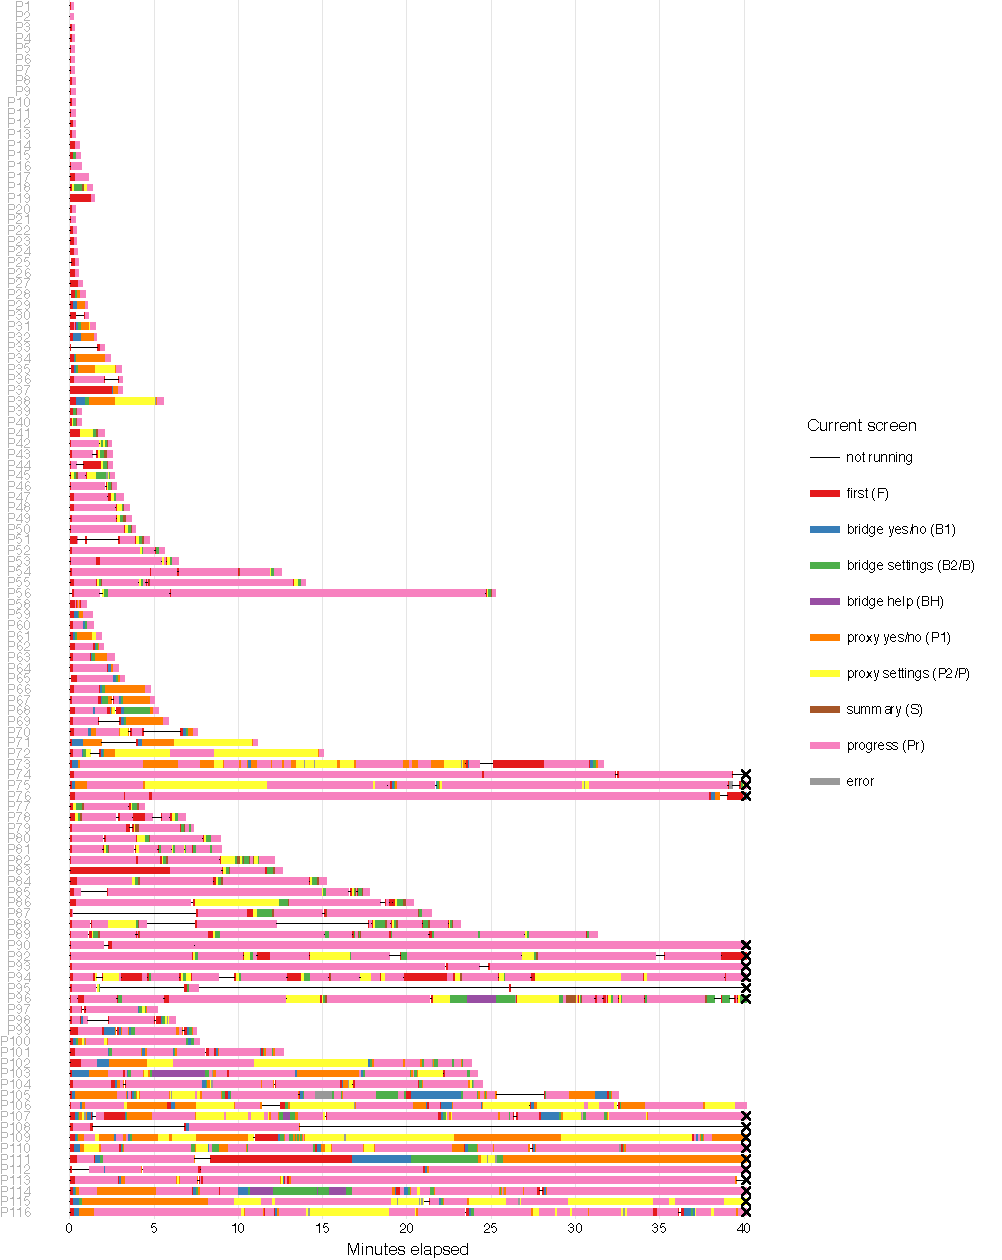
\includegraphics{all-participant-edges}
\caption{
A visualization of our participants' paths through the interface.
The length of the bars show the total time taken to complete the task,
except for those we cut off after approximately 40 minutes.
Different colors indicate which screen they were on during the experiment.
If participants were doing other things (i.e., searching for help in another browser)
while off-focus, this time still counts as spending time in that off-focus window. 
``Not running'' are times when Tor Launcher was closed (i.e., restarting the application).}
\label{fig:all-participant-edges}
\end{figure*}

\subsubsection{Completion Rate} 

\begin{table}[t]
\centering
\begin{tabular}{l r r r r r}
& \multicolumn{2}{r}{completion rate} & \multicolumn{1}{r}{connection} & \multicolumn{1}{r}{configuration} \\
& \multicolumn{2}{r}{(at 40min 8s)} & \multicolumn{1}{r}{time (med)} & \multicolumn{1}{r}{time (med)} \\
\noalign{\hrule}
E1-NEW & 19/19 & 100\% & 0:20 & 0:06 \\
E1-OLD & 19/19 & 100\% & 1:01 & 0:24 \\
E2-NEW & 18/18 & 100\% & 3:22 & 0:40 \\
E2-OLD & 16/19 & 84\% & 5:00 & 2:04 \\
E3-NEW & 13/19 & 68\% & 20:25 & 1:56 \\
E3-OLD & 10/20 & 50\% & 40:08 & 9:09 \\
\end{tabular}
\caption{
An overview of the experiment. 
Those who did not connect were assigned a time of 40:08, 
(the maximum time).
}
\label{table:participant-summary}
\end{table}

Our changes significantly increased success rates (one-tailed Pearson's chi-square test; $\chi^2 = 2.808$, $\mbox{df} = 1$, $p < 0.047$, albeit with small effect size $\phi=0.157$).

Table~\ref{tab:attempts-bridge-proxy} shows participants' connections to Tor. As reported in the first two columns, most participants who did not need to configure anything (E1) didn't, although some optionally used a bridge. Participants who needed any bridge (E2) all used the recommended bridge. Participants who needed a meek-bridge or custom bridge (E3) chose a meek bridge at random; the ones who tried to use a custom bridge did not format their messages or inputs correctly and did not connect to Tor. 

%table
\begin{table}[t]
\centering
% Do not edit this file. Edit attempts.R instead.
\begin{tabular}{r c c c c c c}
& \rotatebox{90}{E1-NEW} & \rotatebox{90}{E1-OLD} & \rotatebox{90}{E2-NEW} & \rotatebox{90}{E2-OLD} & \rotatebox{90}{E3-NEW} & \rotatebox{90}{E3-OLD} \\
no bridge, no proxy & 17 & 13 &  &  &  &  \\
obfs3, no proxy & 2 & 6 & 18 & 16 &  &  \\
meek-amazon, no proxy &  &  &  &  & 7 & 4 \\
meek-google, no proxy &  &  &  &  & 5 & 4 \\
meek-azure, no proxy &  &  &  &  & 1 & 1 \\
no bridge, 3rd-party proxy &  &  &  &  &  & 1 \\
DNF (did not finish) &  &  &  & 3 & 6 & 10 \\
\end{tabular}

\caption{
A table showing participants' connections to Tor.
Note that none used the flashproxy, fte, fte-ipv6, obfs4, or scramblesuit bridges to connect. 
One participant configured a proxy to bypass our simulated censorship environment.
}
\label{tab:attempts-bridge-proxy}
\end{table} 

Seventeen percent (19 of 114) were not able to connect to Tor. The most common reasons for failing to connect were not knowing whether to connect directly or configure a bridge or proxy (P73, P75, P89, P91, P106, P110), not knowing what they needed and trying to configure proxies (P74, P92, P105, P107, P113), and not knowing what to do when a recommended bridge did not work (P90, P93, P108, P111, P114). 


%using http://www.socscistatistics.com/tests/chisquare/Default2.aspx
% OLD VS NEW: The chi-square statistic is 2.8079. The p-value is .093802.
% E1-old vs E1-new: no valid calculation  since it's the exact same ratio (19 succeeded, 0 failed) 
% E2-old vs E2-new: The chi-square statistic is 3.0929. The p-value is .078636.
% E3-old vs e3-new: The chi-square statistic is 1.3666. The p-value is .242403.

\subsubsection{Connection time} 
Our changes significantly reduced connection time (one-tailed Mann--Whitney; $ Z = -1.84$, $p < 0.0328$, $r= 0.172$). We used a one-tailed Mann--Whitney test because the distributions were non-normal, heavily right-tailed, and right-censored. 

However, the simulated censorship environment (and therefore, the difficulty of the configuration), was the strongest factor in determining connection time (Kruskal--Wallis $\chi^2 = 80.5$, $\mbox{df} = 2$, $p < 10^{-15}$). Figure~\ref{fig:time_to_success_clamped} shows that participants in E2 took longer to connect than participants in E1, and participants in E3 took the longest to connect. It would be ideal to have an interface that allows users to connect in the similar amounts of time, no matter what their configuration requirements; neither the OLD or NEW interface achieves this. 

Figure~\ref{fig:time_to_success_ecdf} shows a cumulative distribution of connection times. Everyone in E1 was able to connect right away; participants with the NEW interface doing so faster than participants with the OLD interface. Most participants in E2 were able to connect right away; participants with the NEW interface and OLD interface connecting in a similar distribution of time. Participants in E3 took various amount of time to succeed, with participants with the NEW interface connecting significantly faster than those with the OLD interface. 

\begin{figure}[t]
\centering
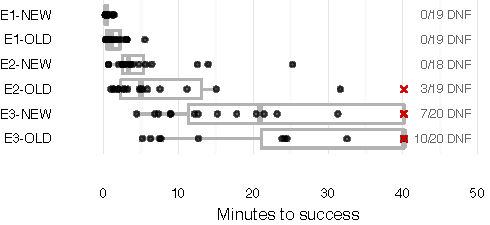
\includegraphics{time_to_success_clamped}
\caption{
Participants in E2 and E3 took a long time to connect.
The ``DNF'' (did not finish) shows how many did not connect.}
\label{fig:time_to_success_clamped}
\end{figure}

\begin{figure}[t]
\centering
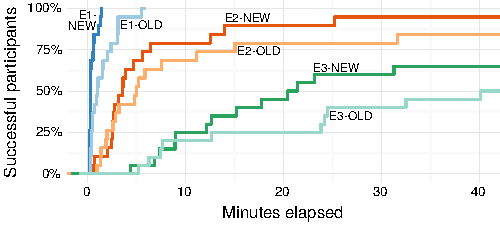
\includegraphics{time_to_success_ecdf}
%../experiment/processing/time_to_success_ecdf.tex
\caption{
Cumulative success rates over time. Those who did not connect were assigned an arbitrarily large finishing time greater than 40 minutes for the purpose of graphing this cumulative distribution. 
}
\label{fig:time_to_success_ecdf}
\end{figure}


\subsubsection{Configuration Time} 
Our changes significantly reduced configuration time (one-tailed Mann--Whitney; $Z = -3.28$, $p < 0.0005$, $r = 0.307$). Again, we used a one-tailed Mann--Whitney test because the distributions were non-normal, heavily right-tailed, and right-censored. 

Figure~\ref{fig:time_to_success_active_clamped} shows that participants' active configuration time were generally a small fraction of their connection time. E1 participants' configuration time was dominated by the time waiting for a connection to be established to Tor because they generally chose the correct configuration right away. E3 participants' configuration time was also dominated by the time waiting for a connection to be established to Tor because they usually needed to try multiple configuration options before connecting, but had to wait for the connection to time out or manually cancel their attempt between attempts. E2 participants' configuration time was a a fraction of their connection time, due to a combination of reasons that affected participants in E1 and E3. 

Due to the reasons above, participants spent a majority of their time on the progress screen compared to the time spent anywhere else (Table~\ref{table:median_time}). We defined configuration time as a participant's connection time spent on all screens but the progress screen, because participants mostly waited on the progress screen. However, we noticed that some participants did utilize this time to search for help in another browser while waiting for their connection to time out, so configuration time is not a prefect metric to measure participant engagement. 

\begin{figure}[t]
\centering
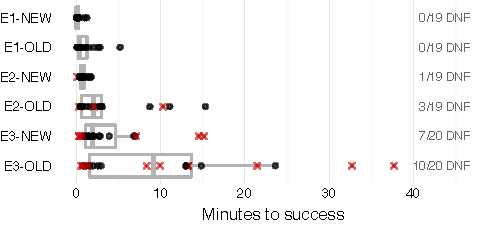
\includegraphics{time_to_success_active_clamped}
\caption{
Configuration times are much shorter than connection times, which means that most of the time was spent waiting for the connection to establish or time out. Non-finishing participants' configuration time was computed by subtracting the time on the progress screen from their assigned completion time.
}
\label{fig:time_to_success_active_clamped}
\end{figure}

\begin{table}[t]
\centering
\begin{tabular}{l r r r r}
& First & Proxy & Bridge & Progress \\
\noalign{\hrule}
E1-NEW & 28\% & 0\% & 0\% & 60\% \\
E1-OLD & 30\% & 0\% & 0\% & 29\% \\
E2-NEW & 6\% & 5\% & 6\% & 78\% \\
E2-OLD & 7\% & 18\% & 8\% & 45\% \\
E3-NEW & 3\% & 5\% & 5\% & 77\% \\
E3-OLD & 2\% & 12\% & 6\% & 64\% \\
\end{tabular}

\caption{
The median percent of time spent on each screen, aggregated over participants in each experimental condition.}
\label{table:median_time}
\end{table}


\section{Recommendations}
\label{sec:recommendations}
Our design resulted in shorter connection times and greater success,  but it could still be improved. We do not recommend our exact design as the optimal design, although we believe it is an improvement. Instead, we offer some suggestions based on what we learned: \\
 
\begin{itemize}
\item {\bfseries Assume users do not know technical concepts.} Users should not need to know what a relay, bridge, proxy, or transport is to connect to Tor. 
\item {\bfseries Explain why users need to make decisions.} Letting users know why they are required to perform a task may make them more sympathetic to  performing that task. For instance, users who need a bridge must choose one manually because different ones work in different countries and Tor does not track users' locations.  
\item {\bfseries Leverage user knowledge.} Users know what country they are connecting from, their level of acceptable risk, and what they are using Tor for. Guiding users to make decisions based on this information will work better than asking about their ISP or explaining what obfuscation protocols are. 
\end{itemize}

We did not try any designs that asked for user inputs, due to design constraints. But we see further room for improvement in success rate, connection time, and configuration time that could be made by leveraging user input and automation. Here, we talk about the potential approaches to redesigning the interface:  \\

\begin{itemize}
\item{\bfseries Design changes:} as demonstrated by our design iteration, tweaks in the interface can result in significant usability improvements.
\item{\bfseries Naive automation:} a scheme that chooses bridges, waits for timeouts, and tries another bridge so users do not need to do this themselves. We call this ``naive'' automation, because this scheme does not leverage information about the user or network conditions and essentially just automates the trial and error process that users would otherwise have to do manually. 
\item{\bfseries Smart automation:} a scheme that connects to a hard-to-censor bridge, which then automatically assigns a bridge that works for the user based on availability and bandwidth constraints. We call this ``smart'' automation because this scheme involves communication with Tor servers, which choose a bridge that will work for the user on the first try. 
\end{itemize}

We recommend a gradual approach that starts with deploying design changes, measuring the impact of those changes, and cautiously incorporating automation into the interface only if the impact of those changes is still unsatisfactory. 

\section{Limitations}
\label{sec:limitations}
We did not study international users, or the interface in languages other than English. All of our participants were from the United States and were instructed to interact with the English version of Tor Browser.

Participants in a laboratory setting may alter their behavior due to their awareness of being observed~\cite{mccarney2007hawthorne}. Ours were likely motivated differently compared to real users. We believe that they were likely over-motivated because they were being observed and receiving a monetary reward. If true, this makes our results a conservative estimate of the usability problems. 

Our experiment did not directly test configuring a proxy or a custom bridge. From observing participants, we suspect they struggle with these tasks. 

We only tested the interface on the Windows operating system. The interface leverages the native operating system's styling and elements, making the configuration interface on Windows look slightly different from the OS~X or Linux equivalents. We acknowledge that participants' unfamiliarity with Windows may have affected our experiment, but we believe that this affected all experimental conditions equally.  

\section{Related Work}
\label{sec:related} 

We do not know of any published usability studies of Tor Browser
since the introduction of Tor Launcher,
which happened in the 3.5 release in December 2013~\cite{torbrowser-35}.
Lee and Fifield ran an informal ``UX sprint''
for Tor Browser in 2015~\cite{uxsprint}, bringing together developers and users
to discover common usability problems.
In what was a precursor to the present work,
they conducted detailed walkthroughs with five participants
to identify common obstacles to using Tor Browser such as hard-to-find downloads,
bad interactions with other end-user security software,
and misleading error messages.

There are studies that evaluated earlier forms of web browsing over Tor,
without a particular focus on configuration.
In 2012, Norcie et~al.~\cite{norcie2012eliminating}
investigated Tor Browser's ``stop-points'' during installation and use,
which they define as places where users' uncertainty about what to do
put them at risk of not completing a task.
Of their 25 participants, 64\% encountered at least one stop-point,
such as a long startup time, misidentified icons, or confusion with other web browsers.

In 2010, Fabian et~al.~\cite{fabian2010privately}
estimated how much Tor's added latency harms usability
(considered separately from user interface concerns).
They measured the latency of requests to common websites with and without Tor,
and mapped the latencies to compute an expected ``cancellation rate,''
which they define as the fraction of users who would have given up waiting for a request to complete.
They estimated a median cancellation rate of 88\% for Tor, compared to 14\% for direct requests.

In 2007, Clark et~al.~\cite{clark2007usability}
used cognitive walkthroughs to evaluate four
methods of web browsing over Tor
(all of which have since been superseded by Tor Browser and Tor Launcher).
Evaluating each method against a set of guidelines,
they found that none were fully satisfactory,
though the ones that used automatic configuration did better.
In 2006, Dingledine and Mathewson~\cite{dingledine2006anonymity}
emphasized that anonymizing networks, by their nature,
require lots of users, so usability is an even greater concern
than with other security systems.

Usable security aims to improve the security of a system by helping the user make good decisions~\cite{payne2008brief}. This involves informing users about the system, communicating risks in a way that is understandable, clarifying what the security requirements are, and providing guidance with technical tasks~\cite{adams1999users}. Usable security research explores a variety of security concepts, such as email encryption~\cite{whitten1999johnny,garfinkel2005johnny}, authentication~\cite{morris1979password,dhamija2000deja,suo2005graphical}, security indicators~\cite{dhamija2006phishing,akhawe2013alice}, and warnings~\cite{schechter2007emperor,egelman2008you}. Our work contributes to this body of knowledge by exploring tools for censorship circumvention.

We used a cognitive walkthrough~\cite{wharton1994cognitive,cognitive-walkthrough} to inspect our interface~\cite{nielsen1994usability}. Other usability inspection methods include heuristic evaluation, pluralistic walkthrough and feature inspection~\cite{inspection}. We used interviews and task benchmarking to get qualitative and quantitative data~\cite{krol2016towards}. Qualitative data can also be collected through focus groups, camera studies, and product surveys. Quantitative data can also be collected through eye tracking, clickstream analysis and A/B testing~\cite{ux-methods}. 
 
For our work, we draw on the large body of previous work in secure interaction design, computer-human interaction, and user studies. Work we found useful to our experiment includes research on principles for secure interaction design~\cite{yee2002user}, common problems in human-computer dialogue design~\cite{molich1990improving}, user tolerance of security delays~\cite{egelmanplease}, treating human attention as a scarce resource when to delegate tasks to users~\cite{bohme2011security}, stopping users from installing potentially harmful programs~\cite{good2007noticing}, and getting proper user consent~\cite{bohme2010trained}. 

\section{Conclusion} 
\label{sec:conclusion}
We measured why and how users have a hard time connecting to Tor through this usability evaluation of Tor launcher. We believe that this is because the interface requires users to know technical terms, provides a lot of freedom for error, and does not give proper feedback. Users in heavily censored environments will likely not succeed in connecting to Tor without outside help. We encourage more usability studies on security tools in general as well as other Tor applications, as they have the potential to create user growth, help user retention, and prevent user frustration. Tor Browser version~5.4.5 incorporated  changes based on our work. We also talked with Tor developers about automating connections to Tor, and they are now considering this as future work. 

\section {Acknowledgments}
We would like to thank the peer reviewers, especially our shepherd Jens Grossklags, for giving us valuable feedback on this paper. Tor Project employees Georg Koppen, Mike Perry, and Isabela Bagueros provided valuable insights about the history of Tor launcher and internal constraints. This work was done in collaboration with Xlab (Experimental Social Science Laboratory)~\cite{xlab}, SCRUB (Secure Computing Research for Users' Benefit)~\cite{scrub}, and BLUES (Berkeley Laboratory for Usable and Experimental Security)~\cite{blues} laboratories, with support from
Intel, the National Science Foundation,
the Open Technology Fund through the Freedom2Connect Foundation, and from
the US Department of State, Bureau of Democracy, Human Rights and Labor.

\bibliographystyle{abbrv}
\bibliography{pets2017-paper.bib}

\appendix

\section{Success and Error States in Tor Launcher 5.0.3} 
\label{states} 
Here we define the end state codes that appear in Figure~\ref{fig:digraph}.
e\# and $\mbox{e\#}^\prime$ are equivalent, except that $\mbox{e\#}^\prime$ uses a bridge while e\# does not. \\

\noindent success states: 
\begin{itemize}
\item s0: no bridge, no proxy
\item s1: valid bridge, no proxy
\item s2: valid bridge and valid proxy (blank port)
\item s3: valid bridge and valid proxy (specified port)
\end{itemize}

error states:
\begin{itemize} 
\item e0: need a bridge or proxy
\item e1: hardcoded bridge blocked
\item e2: custom bridge: field left blank
\item e3: custom bridge: syntax error
\item e4: custom bridge: invalid address
\item e5: custom bridge blocked
\item e6: proxy type is not selected
\item e7: proxy: IP address left blank
\item e8: proxy: syntax error
\item e9: proxy: invalid IP address, blank port
\item e10: proxy: invalid IP address, good port
\item e11: proxy: invalid IP address, bad port
\item e12: proxy: valid IP address, bad port
\item e13: proxy: valid IP address, blank port
\end{itemize} 

The same inputs can lead to different end states,
depending on the network environment.
For example, Tor Launcher will connect to a proxy successfully with the port left blank if the proxy uses port 80 (s2) but will not if the proxy uses another port (e12). 

\section{Qualitative User Study Recruitment Posting} 
\label{qualitative-recruitment}
We are recruiting participants for an in-person research study at the University of California, Berkeley. 
You will need to come in to our lab and perform tasks on a computer for an hour or less. You will be compensated \$30 for participating. 
No special knowledge and no technical experience is required. If you are interested, fill out the survey at \textit{<survey link>}. 

\section{Qualitative User Study Prescreening Survey} 
\label{qualitative-prescreening}
We are recruiting participants for an in-person research study at the University of California, Berkeley. 
You will need to come in to our lab and perform tasks on a computer for an hour or less. You will be compensated \$30 for participating. No special knowledge and no technical experience is required.\\

\begin{enumerate}
\item{Please select when you are available. We will assign you an hour experiment time slot during one of those times.}
\item{I am able to provide my own transportation to the University of California, Berkeley 
campus.}
\item{Thank you for your interest! Please provide an email address where we can contact you to share more logistical details.}
\item{we are looking for a very small number of participants, so unfortunately, we may not be able to accommodate everyone who applies. Would you like us to let you know about future opportunities?}
\item{What is your gender?}
\item{What is your age?}
\item{Please select your highest completed (or current) level of education.}
\item{What is your occupation?} 
\item{Do you speak any languages other than English fluently?}
\item{If you have a personal computer, what kind do you use?}
\item{Which of the following terms have you heard of? \textit{<Answer choices: a checklist of the following terms: malware; proxy services; phishing; SSL; X.511 certificates; Tor.>}}
\item{How often do you use the following software or features? \textit{<Answer choices: a grid of radio buttons. Software/features (rows): HTTPS on web pages; proxies or other censorship circumvention tools; virtual private networks (VPN); file or whole-disk encryption; anonymity systems (e.g., Tor); email encryption (e.g., PGP); chat or instant messaging encryption; voice communication encryption. Frequency (columns): never; less than once a month; a few times a month; several times a week; daily.>}}
\end{enumerate}
Thank you for filling out this form. You are now done!

\section{Qualitative User Study Introduction Script} 
\label{qualitative-script} 
Imagine you live in an oppressive country that censors part of the Internet. We have simulated this in the laboratory by blocking certain websites and services.  The purpose of this experiment is to evaluate the use of Tor browser, which is a browser that can circumvent censorship and let you visit blocked websites. Currently, torproject is blocked (you can check this by going to \begin{NoHyper}\url{torproject.org}\end{NoHyper} on a standard browser, like Firefox, Chrome, or Internet Explorer). 

To circumvent censorship successfully, you will need to set up Tor browser correctly and use it to get to Wikipedia. If you are able to reach the website, then you know that you have successfully circumvented censorship. Fill out the question on the worksheet. This isn't intended to be hard, just write what you see. We want to just check you saw the website. 

Before you start, do you have any questions about what you are asked to do? 

\section{Qualitative Study Worksheet Text} 
\label{participant-worksheet}
Imagine you live in an oppressive country that censors part of the Internet. We have simulated this in the laboratory by blocking certain websites and services. The purpose of this experiment is to evaluate the use of Tor browser, which is a browser that can circumvent censorship and let you visit blocked websites. For instance, \begin{NoHyper}\url{www.torproject.org}\end{NoHyper} is blocked. Check this by going to the site on a standard browser, like Firefox, Chrome, or Internet Explorer. It will fail to load, when you can visit other sites.

To complete this worksheet, you will need to set up Tor browser (on your desktop) correctly and use it to get to blocked site. If you can visit wikipedia, then you know that you have successfully circumvented censorship.

\section{Post-Experiment Standard Interview Questions}
\label{interview-questions}
We asked our participants these questions after they were given time to configure Tor Browser. \\

\begin{enumerate}
\item{Can you talk us through what you did along with what you were thinking at the time?}
\item{What was most challenging part of connecting?}
\item{Were there any unfamiliar terms?}
\item{How did you decide which options to choose?}
\item{What did you think about using Tor?}
\item{What is one change you would recommend?} 
\item{Did you need any additional information?} 
\end{enumerate}  

In addition to these questions, we asked our participants about specific questions based on their observation, usually regarding a specific choice in action, a particular screen they seemed stuck on, and any errors they encountered during the configuration process. 

\section{Qualitative Testing Observations}
\label{summary}
We summarize each participant's session.

%E1: P2, P3, P4, P9, P10
%E2: P7, P8, P11, P12, P13
%E3: P1, P5, P6, P14, P15, P16

% re-watched the videos and get the exact times. 
%https://github.com/lindanlee/PETS2017-paper/tree/master/sessions/pre/videos

\subsection{E1} 
In E1, any connection to Tor worked. Configuring bridges and proxies was optional.  
Observations in E1: 

%P9 (regular): E1 (0:39; 4:49 to 5:28)
\pquote{P1 (new user, direct, 0:39)}{They connected directly.}

%P2(regular): E1 (1:20, 0:22 to 1:42) 
\pquote{P2 (new user, direct, 1:20)}{They spent time reading the text on the start screen, and connected directly because they were intimidated by the other option.}

%P3(regular): E1 (N/A; 5:47 to 6:26) 
\pquote{P3 (new user, obfs3, 1:39)}{They connected with the recommended bridge. They were also going to use a proxy, but decided not to when they saw the proxy input fields.}

%P4(regular): E1 (8:56, 7:22 to 16:18)
\pquote{P4 (new user, obfs4, 8:56)}{They chose the recommended bridge and then tried to configure a proxy. After not being able to fill out the proxy input fields, they started over and connected with an obfs4 bridge. Note that they did not try connecting with the obfs3 bridge, which would have worked.}

%P10 (has used Tor before): E1 (1:02; 0:13 to 1:15)
\pquote{P5 (previous Tor user, obfs3, 1:02)}{They connected with the recommended bridge.}

Participants in E1 were able to connect to Tor, but most were unsure if their actions were correct. Three of the five participants unnecessarily configured bridges. 

\subsection{E2} 
In E2, a bridge was required to connect. Any of the hardcoded bridges from the dropdown menu, as well as any custom bridges acquired out of band would work. Configuring a proxy was optional.
Observations in E2: 

%P7 (heard of Tor): E2 (4:04; 0:29 to 4:33) 
\pquote{P6 (new user, obfs3, 4:04)}{They tried connecting directly. After watching the progress bar not make any progress for a couple minutes, and gave up on the direct connection. Then they connected with the recommended bridge.}

%P13 (regular): E2 (7:48; 0:34 to 9:22) 
\pquote{P7 (new user, obfs3, 9:22)}{They tried connecting directly. They restarted Tor Launcher and tried to connect directly again---and repeated this two more times. On the fourth restart, they tried to configure a proxy, but gave up. On the fifth restart, they connected using the recommended bridge.}

%P12 (regular): E2 (10:40; 0:46 to 11:26)
\pquote{P8 (new user, direct, 10:40)}{They tried connecting directly. After waiting a couple minutes, they figured that did not work and looked at proxy settings. But after looking at the settings and being intimidated, they tried connecting directly again. Then, they tried to configure a proxy, and gave up. They tried connecting directly again, which worked unexpectedly. They found a bug in our setup that we fixed for the later experiment. E2 required a bridge to connect, but new public relays came online after we ran our firewall rules and they were able to connect using those new relays. }

%P11 (used Tor before): E2 (~3:00; 1:05 to 5:13)
\pquote{P9 (previous Tor user, obfs3, 4:08)}{They tried connecting directly. And they tried connecting directly through a different user path by answering `no' to the bridge and proxy questions in the interface, connecting from the proxy screen. Then, they connected using the recommended bridge.}

%P8 (used Tor): E2 (clock drift mission impossible, 1:38 to 7:20) 
\pquote{P10 (previous Tor user, failed to connect)}{They tried a direct connection. Then, they tried a connection with the recommended bridge, which should have worked. However, our setup experienced a clock drift. Tor does not allow connections with bad clocks. They spent the rest of their time trying different bridges and proxies in vain (Figure~\ref{fig:proxy-attempt}). This participant made the most connection attempts, using a variety of bridges and proxies.}

Participants in E2 tried a direct connection to Tor before \emph{eventually} connecting with the recommended bridge.
They spent a fair amount of time waiting before determining that connections failed. Some stated that they connected directly because the interface says that it would work in ``most situations'' (Figure~\ref{fig:old-first}). Our participants did not know if they needed bridges or proxies, so they only tried to configure one when the direct connection failed. Since they did not know whether they needed a bridge or proxy, they often tried to configure proxies when they did not need one and should have configured bridges instead.  

\subsection{E3}
In E3, a bridge was required to connect. Most of the hardcoded bridges in the dropdown menu would not work, with the exception of meek-amazon, meek-azure, and meek-google. Custom bridges can also work. Configuring a proxy was optional.
Observations in E3: 

\begin{figure}[t]
\centering
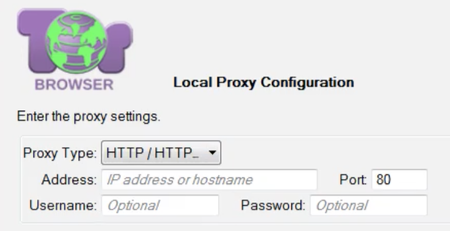
\includegraphics[width=0.5\textwidth]{P8-proxy-attempt.png}
\caption{
Proxies were not necessary to connect to Tor, but many spent time trying to configure one when they couldn't connect. Here, we show P10's unsuccessful attempt. 
}
\label{fig:proxy-attempt}
\end{figure}

%P14 (regular): E3 FAIL
\pquote{P11 (new user, failed to connect)}{They tried connecting directly, and then with the recommended bridge. Then, they retried connecting directly and retried connecting using the recommended bridge. After that, the participant spent the rest of their time trying to configure a proxy and retrying connections with the recommended bridge.}

%P15 (regular): E3 FAIL
\pquote{P12 (new user, failed to connect)}{They tried connecting with the recommended bridge. They decided that they need a proxy along with the recommended bridge, and spent the rest of their time trying to configure a proxy.}

%P16: E3 (regular) FAIL
\pquote{P13 (new user, failed to connect)}{They tried connecting directly, and then with the recommended bridge. They retried connecting with the recommended bridge. When that didn't work, they tried to configure a proxy. Then, they gave up on the task entirely.}

%P6 (heard of Tor): E3 (26:48; 0:18 to 27:06) 
\pquote{P14 (new user, meek-google, 26:48)}{They tried a direct connection by answering `no' to the bridge and proxy questions. After waiting a while, they canceled the connection and tried connecting with the recommended bridge. They retried connecting with the recommended bridge two more times, then tried to connect with a flashproxy bridge, an obfs4 bridge, a scramblesuit bridge. After retrying the recommended bridge again, they made a connection using a meek-google bridge.}

%P1 (heard of tor before): E3 (~7:31, 0:51 to 8:22) 
\pquote{P15 (new user, meek-azure, 7:31)}{They tried connecting directly, and then with the recommended bridge. After that, they tried a connection using a meek-azure bridge, but gave up after before it could connect. They went back to the first screen (Figure~\ref{fig:old-first}) and clicked connect, which made a connection using a meek-azure bridge. The connect button makes a connection to Tor with the toggled settings in the interface. When the interface is initialized to not use a bridge or proxy, clicking connect on the first page starts a direct connection. But since the participant had chosen a meek-azure bridge, the connect button made a connection to a meek-azure bridge, even though the text in the first screen says that they will ``connect directly.'' Because of this, the participant thought they made a direct connection. Although they succeeded in connecting to Tor, they did not realize what they had done or why connecting to a meek-azure bridge worked. They chose that bridge at random.}

%P5 (has used tor before): E3 (22:06; 0:00 to 22:06)
\pquote{P16 (previous Tor user, custom bridge, 22:06)}{They tried and retried connecting directly, then they tried connecting with the recommended bridge. After briefly looking at error messages in the system log, they retried connecting directly two more times. After trying to configure a proxy for a while, they instead decided not to use one and tried connecting with a meek-google bridge, which would have worked. But  due to a bug in the progress bar that prevents it from updating correctly on subsequent attempts, they gave up before it could connect. They made a connection with the custom bridge by following the instructions from the bridge help button (they created a throwaway email account, emailed the bridge responder with poor syntax and did not get a response, emailed the bridge responder again with correct syntax and got a response, and then typed in the bridge information into the custom bridge field).}

Participants in E3 also generally tried a direct connection to Tor. They did not know if they needed a bridge or proxy, and like the participants in E2, only configured them when the direct connection failed. Of the participants that failed, they all tried the recommended bridge but not any others. The participants that did manage to connect to Tor did not know which bridges worked and which ones did not, or which ones to try next in case the recommended one failed. P14 brute-forced options until something worked, P15 did not think that they were using a bridge, and P16 gave up on a hardcoded bridge that would have worked and used a custom bridge instead.

\section{Quantitative User Study Recruitment Posting}
\label{quantitative-recruitment}
We are recruiting up to 40 participants for a user study at UC Berkeley. 
The experiment will involve basic Internet browsing tasks. You are not eligible if you have participated in our previous sessions.\\

\indent Payment: \$30 Amazon gift card\\
\indent Duration: 1 hour \\
\indent Where: Xlab at Hearst Memorial Gymnasium\\

\textit{<list of sessions>}\\

To be eligible, you must be an adult (18 or older). This is to comply with university policies on research. 

If you are interested: 1.~Email lnl@berkeley.edu 
with the sessions you are able to attend. We will confirm your participation and assign you a session. 
2.~Come to Xlab 
at the appointed time for the experiment.

\section{Quantitative User Study Introduction Script} 
\label{quantitative-script} 
Imagine you live in an oppressive country that censors part of the Internet. We have simulated this in the laboratory by blocking certain websites and services.  The purpose of this experiment is to evaluate the use of Tor browser, which is a browser that can circumvent censorship and let you visit blocked websites. Currently, torproject is blocked (you can check this by going to torproject.org on a standard browser, like Firefox, Chrome, or Internet Explorer). 

To circumvent censorship successfully, you will need to set up Tor browser correctly and use it to get to Wikipedia. Tor is already installed for you. On the desktop, you should see a globe icon that says ``Start Tor Browser.'' If you are able to reach the website, then you know that you have successfully circumvented censorship. Fill out the question on the worksheet. This isn't intended to be hard, just write what you see. We want to just check you saw the website. 

Afterward, we ask you to take a short survey to collect some information about you. The link is also on your worksheet.
We will give you time to complete this task. If you finish early, we ask that you sit at your desk until the remainder of the hour. Since we are recording your screen, we ask that you don't do anything personal afterward, like checking your email.

Before you start, do you have any questions about what you are asked to do? 

\section{Quantitative User Study Worksheet Text} 
\label{summative-worksheet}
Imagine you live in an oppressive country that censors part of the Internet. We have simulated this in the laboratory by blocking certain websites and services.

The purpose of this experiment is to evaluate the use of Tor browser, which is a browser that can circumvent censorship and let you visit blocked websites. For instance, www.torproject.org is blocked. Check this by going to the site on a standard browser, like Firefox, Chrome, or Internet Explorer. It will fail to load, when you can visit other sites.

To complete this worksheet, you will need to set up Tor browser (on your desktop) correctly and use it to get to blocked site. If you can visit wikipedia, then you know that you have successfully circumvented censorship.

\begin{enumerate}
\item Visit Wikipedia's main page (\begin{NoHyper}\url{https://en.wikipedia.org/wiki/Main_Page}\end{NoHyper}). What is the topic of today's selected article?
\item After you have completed the tasks, fill out this survey: \begin{NoHyper}\url{http://bit.ly/tor-survey}\end{NoHyper}
\end{enumerate}


\section{Quantitative User Study Exit Survey} 
\label{quantitative-exit-survey}
We'd like to know more about you.  All of your answers will be stored separately from any identifying information in order to protect your confidentiality.

This survey is part of a research project being conducted by the University of California, Berkeley. 
If you have any questions about your rights or treatment as a research participant in this study, please contact the University of California at Berkeley's 
Committee for Protection of Human Subjects at 510-642-7461, or email 
subjects@berkeley.edu. 
If you agree to participate, please click Next below.\\

\begin{enumerate}
\item{What is your participant ID? (This can be found on the sticker on the left hand corner of the desk you are currently sitting at.)}
\item{What is your gender?}
\item{What is your age?}
\item{Please select your highest completed (or current) level of education}.
\item{What is your current occupation?}  
\end{enumerate}

Thank you for participating in our experiment. You are now done! Please sit at your desk for the remainder of the experiment. Our researchers will formally announce the end of the experiment. 


\end{document}
